\documentclass{beamer}[fontset=windows]
\usepackage{ctex, hyperref}
\usepackage[T1]{fontenc}
\usepackage[backend=bibtex,bibstyle=gb7714-2015,citestyle=gb7714-2015]{biblatex}
\addbibresource{ref.bib}
\setlength{\bibitemsep}{3bp}
\renewcommand*{\bibfont}{\zihao{5}\linespread{1.27}\selectfont}
\usefonttheme[onlymath]{serif}
% other packages
\usepackage{latexsym,amsmath,xcolor,multicol,booktabs,calligra}
\usepackage{graphicx,pstricks,listings,stackengine}

\author{吴熙楠}
\title{钙钛矿材料}
\institute{北京大学物理学院}
\date{\today}
\usepackage{PKU}
\logo{
\includegraphics[scale=0.025]{pic/PKU_logo.png}}
% defs
\def\cmd#1{\texttt{\color{red}\footnotesize $\backslash$#1}}
\def\env#1{\texttt{\color{blue}\footnotesize #1}}
\definecolor{deepblue}{rgb}{0,0,0.5}
\definecolor{deepred}{rgb}{0.6,0,0}
\definecolor{deepgreen}{rgb}{0,0.5,0}
\definecolor{halfgray}{gray}{0.55}

\lstset{
	basicstyle=\ttfamily\small,
	keywordstyle=\bfseries\color{deepblue},
	emphstyle=\ttfamily\color{deepred},    % Custom highlighting style
	stringstyle=\color{deepgreen},
	numbers=left,
	numberstyle=\small\color{halfgray},
	rulesepcolor=\color{red!20!green!20!blue!20},
	frame=shadowbox,
}


\begin{document}
	
	\kaishu
	\begin{frame}
		\titlepage
	\end{frame}
	
	\begin{frame}
		\tableofcontents[sectionstyle=show,subsectionstyle=show/shaded/hide,subsubsectionstyle=show/shaded/hide]
	\end{frame}
\section{金属卤化物钙钛矿及其性质}
\subsection{金属卤化物钙钛矿的基本概念}
\begin{frame}
	\begin{itemize}
		\item 1839年德国矿物学家 Gustav Rose 发现了$ CaTiO_{3}$矿石,并以俄国矿物学家 LevPerovski的名字命名(Perovskite)。
		\item 金属卤化物钙钛矿结构通式也符合$AMX_{3}$,但A位离子主要是甲铵($MA^{+}$)、甲脒($FA^{+}$)或者铯($Cs^{+}$)等一价阳离子,M 位离子主要 IV 主族的二价铅($Pb^{2+}$)或锡($Sn^{2+}$)离子,X位主要是负一价卤素离子,包括 $Cl^{-}$, $Br^{-}$和 $I^{-}$。
	\end{itemize}
	\begin{figure}[H]
	\centering
	\hspace{2em}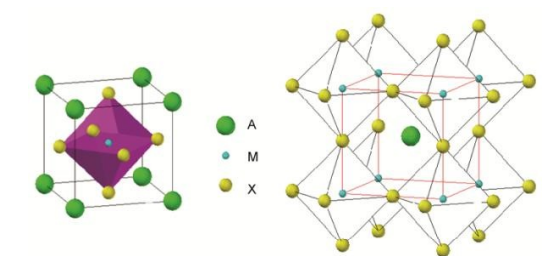
\includegraphics[width=.65\linewidth]{pic/1.png}
	\caption{金属卤化物钙钛矿结构示意图
	}
\end{figure}
\end{frame}
\subsection{金属卤化物钙钛矿的基本光学性质}
\begin{frame}
	\begin{itemize}
		\item 作为一种晶体半导体材料,金属卤化物钙钛矿的一大显著优势是发光可以在$400-800 nm$ 的范围内连续可调,覆盖了整个可见光区域\cite{stranks2015metal}。最常见的调节钙钛矿发光峰位的方法是改变钙钛矿元素种类,A, M, X 三种离子的选取对钙钛矿的能带结构都有一定影响,从而导致发光峰位的移动\cite{sutherland2016perovskite}。
		\item 如$ CsPbI_{3}$钙钛矿的禁带宽度是$1.73eV$\cite{swarnkar2016quantum},$CsPbBr_{3}$钙钛矿的禁带宽度是$2.35 eV$\cite{becker2018bright}, $CsPbCl_{3}$ 钙钛矿的禁带宽度则达到 $3.06 eV$\cite{becker2018bright}。通过选择合适卤素元素并适当混合(如 $CsPb(Cl/Br)_{3}$,$CsPb(Br/I)_{3}$等),就可以得到发光覆盖$400-700nm$的$CsPbX_{3}$ 钙钛矿。
		\item 钙钛矿材料大部分为宽禁带半导体材料,除了光学性质外还有很好的热导率,击穿场强及电子饱和迁移速率。
	\end{itemize}
\end{frame}	
\begin{frame}
	\begin{figure}[H]
		\centering
		\hspace{2em}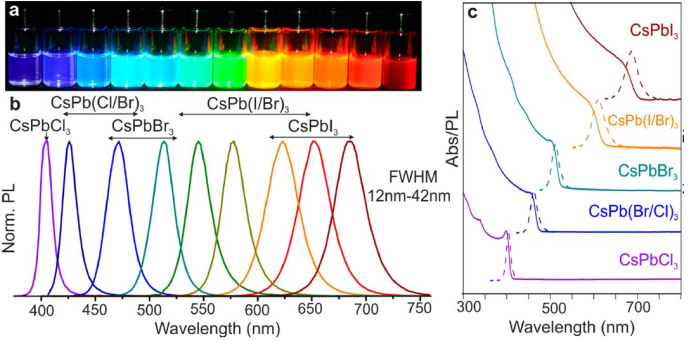
\includegraphics[width=.75\linewidth]{pic/2.png}
		\caption{$CsPbX_{3}$钙钛矿组分调控实现光谱调控\cite{yakunin2015low}
		}
	\itshape
	$a.$紫外灯$365 nm$下的 $CsPbX_{3}$ 钙钛矿溶液照片;$b.CsPbX_{3}$钙钛矿的荧光光谱;$c.$典型$ CsPbX_{3} $钙钛矿的吸收与荧光光谱
	\end{figure}
\end{frame}
\begin{frame}
	\begin{itemize}
		\item 金属卤化物钙钛矿的另一个重要的优点是窄发光峰宽带来的高色纯度。作为一种直接带隙半导体材料,钙钛矿的荧光来自于带边自由载流子的直接复合(如三维钙钛矿,激子束缚能较小,基本不受到晶体尺寸的影响)或带边激子直接复合(纳米结构钙钛矿,激子束缚能较大的情况),因此钙钛矿的荧光半峰宽非常窄。
	\end{itemize}
	\begin{figure}[H]
	\centering
	\hspace{2em}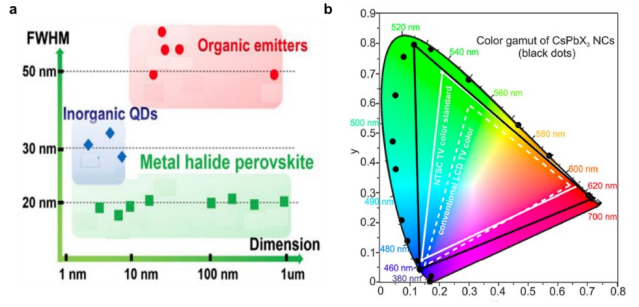
\includegraphics[width=.7\linewidth]{pic/3.png}
	\caption{$a.$钙钛矿、量子点、有机发光材料的半峰宽对比;$b.$钙钛矿发光材料色域覆盖范围\cite{yakunin2015low}
	}
\end{figure}
\end{frame}
\begin{frame}
	\begin{block}{荧光量子产率}
		\begin{itemize}
			\item 单位时间内,发光材料发射的光子数与吸收的光子数之比。
			\item 考虑到材料吸收光子产生的激发态(自由载流子和激子等)最终会通过各种辐射复合通道和非辐射复合通道复合。$PLQY=\dfrac{k_{r}}{k_{r}+k_{nr}}$
			\item 辐射复合:是自由载流子的双分子复合也可以是电子空穴对形成激子后的单分子复合;非辐射复合:各种缺陷和陷阱态造成的单分子复合,在激发密度很高的情况下,俄歇复合也会造成严重的非辐射复合。
			\item 钙钛矿量子点由于量子限域效应,激子束缚能较大,同时俄歇复合常数较小,因此在得到较好的表面钝化过后会量子产率非常高,接近$100\%$\cite{li2016cspbx3}(其余荧光LED材料在激发浓度较小时$PLQY$会明显下降)。
		\end{itemize}
	\end{block}
\end{frame}
\section{钙钛矿二极管}
\subsection{钙钛矿二极管基本构成}
\begin{frame}
	\begin{block}{$PeLED$结构}
		\begin{itemize}\small{
			\item 一个完整的 $PeLED$ 器件至少有以下五个功能层组成,依次包括阴极、电子传输层、钙钛矿发光层、空穴传输层和阳极。
			\item 阴极材料负责向电子传输层注电子,一般以低功函数的材料,如 $Ca, Al,Ag$ 等金属较为多见。
			\item 电子传输层将阴极注入的电子传输并注入到发光层,要求电子迁移率高,导带 位置合适,常见的有$ ZnO,TiO_{2} $等氧化物纳米晶或者部分小分子有机物材料。
			\item 发光层为钙钛矿,注入的电子和空穴在此复合,因此要求荧光量子产率尽量高,同时价带导带能级位置合适以满足载流子平衡注入的要求。
			\item 空穴传输层将阳极注入的空穴运输并注入到发光层,因此要求空穴迁移率高,价带位置合适,常见的有$ NiO$及部分有机物材料。
			\item 阳极负责向空穴传输层注入空穴,一般要求高功函数的材料,常见有铟锡氧化物透明导电薄膜($ITO$),氟掺杂的 $SnO_{2}$透明导电薄膜(FTO)和金属 $Au $等。}
		\end{itemize}
	\end{block}
\end{frame}
\begin{frame}
	\begin{figure}[H]
		\centering
		\hspace{2em}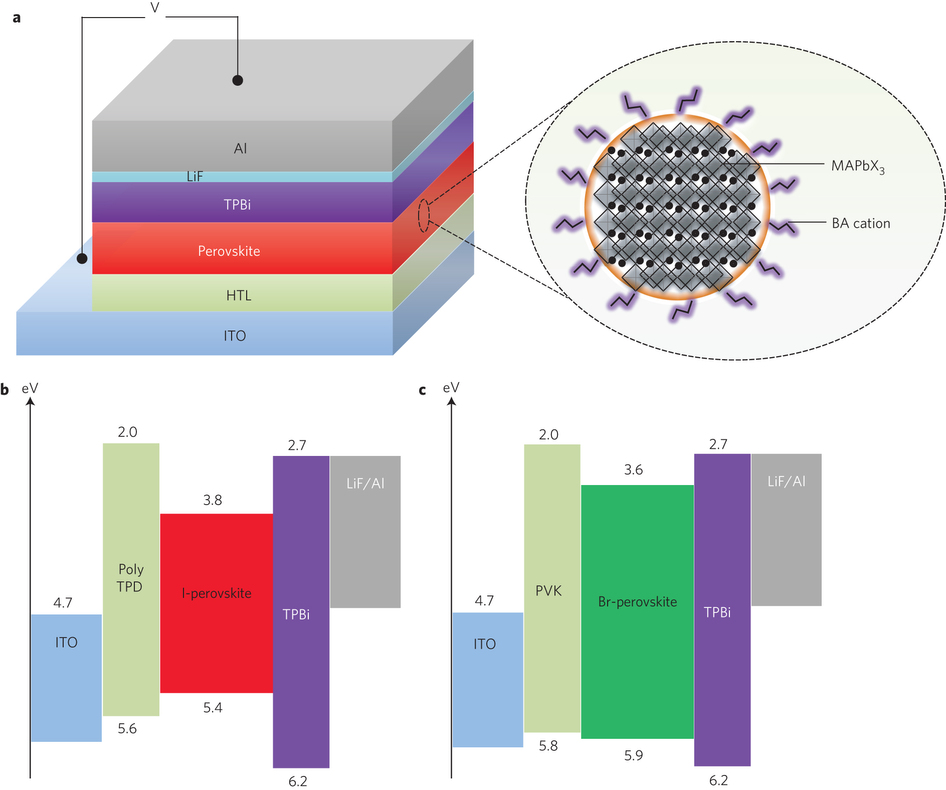
\includegraphics[width=.75\linewidth]{pic/6.jpg}
		\caption{钙钛矿发光二极管结构图及能量图
		}
	\end{figure}
\end{frame}
\begin{frame}
	\begin{block}{$PeLED$工作原理}
		\begin{itemize}\small{
			\item 注入的电子和空穴在发光层中相遇,形成激子后发生辐射复合或电子和空穴作为自由载流子直接发生双分子复合最后复合产生的光子穿过各个功能层后射出器件。
			\item 钙钛矿层的折射率一般比较大(如$FAPbI_{3}$ 折射率为 $2.7$),且通常钙钛矿材料发光是各向同性的,因此,考虑到全反射条件的限制,将有很大一部分辐射出来的光子无法射出器件。
			\item $PeLED$ 器件的总厚度往往不超过 $300 nm$,发光中心到金属电极的距离小于半波长。此时 $PeLED$ 中将出现明显的近场光学效应,金属电极会带来强烈的表面等离子共振吸收,造成大量光损耗。
			\item 钙钛矿消光系数很高($\sim 10^{4}cm^{-1}$),在部分钙钛矿比较厚的 $PeLED$ 器件中存在显著的自吸收现象,也可能会造成光子的消耗\cite{cho2020role}。 
			\item 目前在每层不增加任何光提取情况下能达到最大出光效率为$20\%\sim 30\%$
		}
		\end{itemize}
	\end{block}
\end{frame}
\subsection{钙钛矿二极管的特点}
\begin{frame}
	\begin{itemize}\small{
		\item  $PeLED$发光层的沉积过程伴随着钙钛矿的形成与结晶的过程,薄膜沉积工艺不但影响钙钛矿薄膜的形貌,也极大地影响着钙钛矿膜的发光性质($OLED$ 与 $QLED$ 都需要先合成发光材料,然后再蒸镀、旋涂、喷墨打印等方法沉积成发光层,沉积过程原则上只影响发光层的形貌而不会影响发光性质)。
		\item $PeLED$的离子迁移问题(钙钛矿器件稳定性差的罪魁祸首):由于钙钛矿本质上是一种离子晶体,当有外加电场存在时,钙钛矿中的离子(主要是卤素离子)会从晶体结构比较“脆弱”的地方,如晶界、表面等存
		在大量缺陷的地方开始发生移动,从而导致器件性能的衰减\cite{wang2016stability}(解决方法暂时只有表面处理钝化)。
		\item $PeLED$的迟滞现象:受到离子迁移的影响,$PeLED$ 的电流-亮度-电压曲线和效率-电压曲线在正扫和反扫是不重合的(解决方法暂时也只有表面处理钝化)。
	}
	\end{itemize}
\end{frame}
\begin{frame}
	\begin{figure}[H]
		\centering
		\hspace{2em}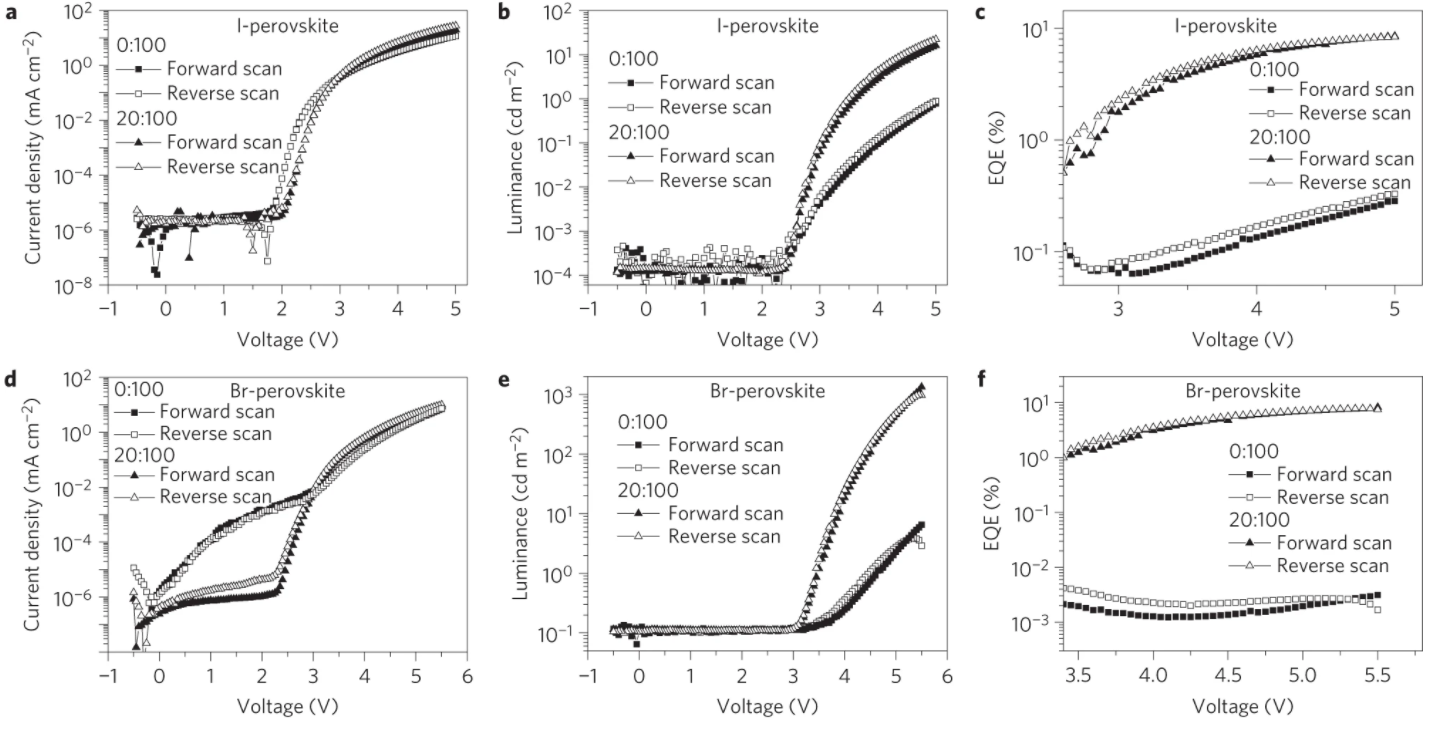
\includegraphics[width=1.0\linewidth]{pic/4.png}
		\caption{迟滞效应对$PeLED$性能的影响\cite{xiao2017efficient}
		}
	\end{figure}
\end{frame}
\subsection{$PeLED$与$OLED$和$QLED$对比}
\begin{itemize}\small{
	\item 光谱方面,$PeLED$ 和 $QLED$ 都可以通过组分调节以及量子限域效应的方法改变发光峰位,电致荧光可以从整个可见光范围延伸到近红外区域。$OLED$ 要实现发光峰位的移动则需要合成不同的发光分子,光谱范围基本集中在可见光区域。
	\item 色纯度方面,由于有机材料固有限制,$OLED(FWHW>50 nm)$ 比 $QLED$($FWHW\sim 30 nm$)和$PeLED$($FWHW< 20 nm$)都要略逊一筹,因此$PeLED $在色纯度方面表现尤其出色,能够覆盖更广的色域空间,非常适合用于高性能显示器件。
	\item 器件方面,$OLED$ 的最高效率往往在低亮度下达到,高电流高亮度情况下则伴随着显著的效率滚降,而 $QLED$ 和$PeLED$ 都报道了效率滚降很小的器件,满足了高亮度场景的使用要求。($OLED$ 与$QLED$ 目前都已经有超过百万小时寿命的器件报道,$OLED$ 更是已经投入了商业化应用,而$PeLED$的稳定性研究才刚刚起步不久,报道的最佳寿命也仅仅数百小时\cite{wang2019trifluoroacetate}。)
	\item 工艺方面,三种器件都可以通过低成本的低温溶液加工工艺生产制备,都可以兼容柔性衬底,而$OLED$ 除了溶液工艺之外还可以通过真空蒸镀的方式制备。
}
\end{itemize}
\begin{frame}
	\begin{figure}[H]
		\centering
		\hspace{2em}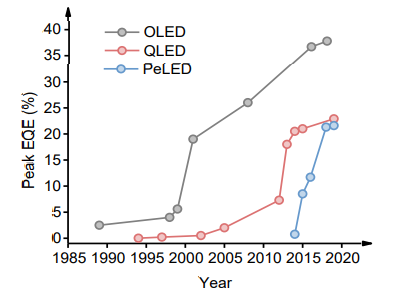
\includegraphics[width=.8\linewidth]{pic/5.png}
		\caption{$OLED, QLED, PeLED $效率发展历程
		}
	\end{figure}
\end{frame}
\subsection{钙钛矿二极管发展历程}
\begin{itemize}
	\item 1994年,日本九州大学团队第一次利用钙钛矿进行电致发光,但由于激子声子相互作用很强,只能在极低温使用。
	\item 2014 年,剑桥大学 Richard Friend 团队率先报道了室温下可工作的钙钛矿 LED。
	\item 2015 年南工大王建浦与浙大金一政团队合作研究,将 $PeLED$ 的效率提升到了 $0.8\%$(绿
	光)和 $3.5\%$(近红外)。
	\item 2017 年,普林斯顿大学 Barry Rand 等人发现通过精细调控钙钛矿前驱体溶液中加的长链铵盐的
	量,除了准二维钙钛矿之外,还可以形成自组装的钙钛矿纳米晶。
	\item 2018 年南工大王建浦团队实现了最高$ EQE$ 达到 $20.7\%$的近红外$PeLED$。
	\item 2018年华侨大学魏展画团队实现了最高 $20.3\%EQE$ 的绿光 $PeLED$。
	\item $\cdots$
\end{itemize}
\subsection{钙钛矿二极管主要问题}
\begin{frame}
	\begin{block}{蓝光$PeLED$}
		\begin{itemize}
			\item 混合卤素方法来调整材料的带隙,实现蓝光发射,在电场和强光照等激发条件下会出现比较严重的离子迁移现象,从而造成发光光谱随着不同偏压和不同工作时间的变化而逐渐红移,光谱稳定性不好。
			\item 利用量子限域效应通过降低材料维度将绿光波段移动到蓝光波段,但此方法对于材料制备比较严苛,条件稍微改变将会引起较大改变。
			\item 虽然在溶液中钙钛矿纳米晶有较高的$PLQY$,但在转移成膜后由于配体不稳定等因素会造成$PLQY$的下降。
			\item 为保证钙钛矿纳米结构的稳定,制备过程一般会配体过量,但大量的配体会阻碍电子空穴运输。
		\end{itemize}
	\end{block}
\end{frame}
\begin{frame}
	\begin{block}{$PeLED$的稳定性}
		\begin{itemize}
			\item 目前报道的$PeLED$器件最稳定均在近红外波段,在可见光范围的工作时间很短(器件寿命一般为几百小时),尤其是蓝光范围器件寿命甚至是分钟级别的,远不如$OLED,QLED$稳定。
			\item 钙钛矿为离子晶体,在加热/强光照/强电场条件下,钙钛矿的晶界、表面等缺陷较多的位置会启动离子迁移过程,从而导致器件性能的衰减。
			\item 目前制作半导体太阳能电池的工作电极会向器件内部扩散,而扩散的金属离子会进入钙钛矿的深能级复合中心,破坏钙钛矿的发光性能。
		\end{itemize}
	\end{block}
\end{frame}
\section{钙钛矿材料的其他应用}
\begin{frame}{钙钛矿太阳能电池}
	\begin{figure}[H]
		\centering
		\hspace{2em}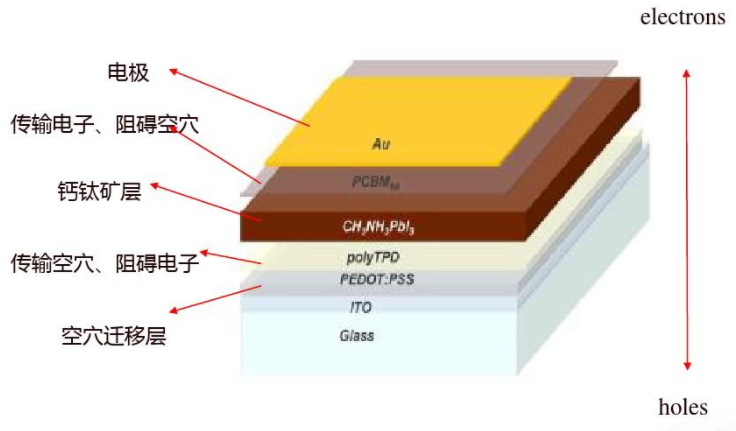
\includegraphics[width=.8\linewidth]{pic/6.png}
		\caption{钙钛矿太阳能电池结构图
		}
	\end{figure}
\end{frame}
\begin{frame}{钙钛矿纳米激光器}
	\begin{figure}[H]
		\centering
		\hspace{2em}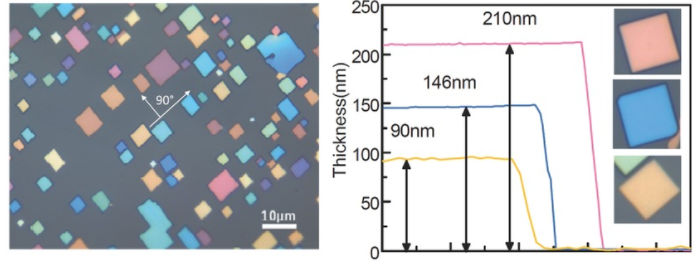
\includegraphics[width=.8\linewidth]{pic/7.png}
		\caption{钙钛矿单晶薄膜示意图\cite{zhang2016high}
		}
	\end{figure}
\end{frame}
\begin{frame}
	\begin{figure}[H]
		\centering
		\hspace{2em}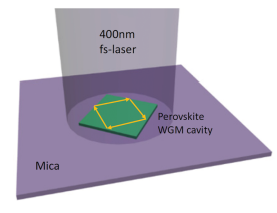
\includegraphics[width=.7\linewidth]{pic/8.png}
		\caption{$CsPbBr_{3}$实现$WGM$模式激光\cite{zhang2016high}
		}
	\end{figure}
\end{frame}
\begin{frame}{钙钛矿光电探测器}
	\begin{figure}[H]
		\centering
		\hspace{2em}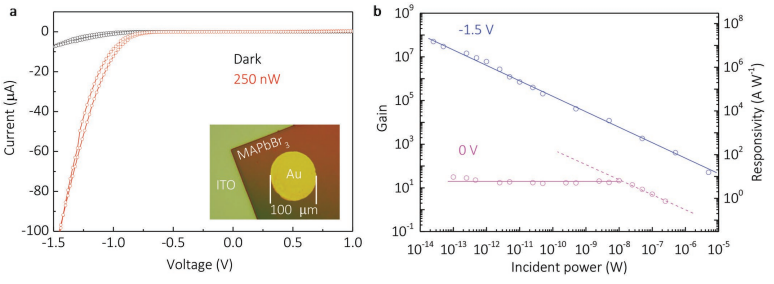
\includegraphics[width=1.0\linewidth]{pic/9.png}
		\caption{$a.$黑暗与照明情况下探测器的电流电压曲线;$b.$器件的增益与响应度\cite{yang2018high}
		}
	\end{figure}
\end{frame}
\begin{frame}{钙钛矿燃料电池}
	\begin{figure}[H]
		\centering
		\hspace{2em}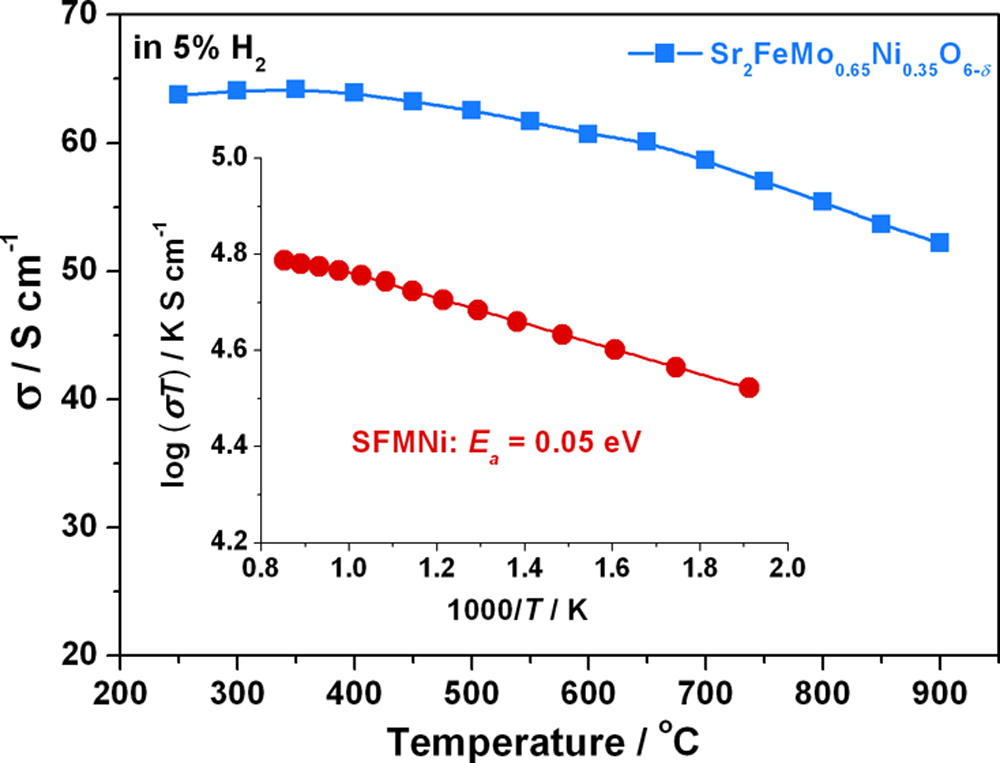
\includegraphics[width=.7\linewidth]{pic/1.jpeg}
		\caption{单电池氢气气氛测试不同温度,电压以及功率密度和电流密度的曲线图\cite{du2016high}
		}
	\end{figure}
\end{frame}
\section{总结}
\subsection{钙钛矿材料的优势}
\begin{frame}
\begin{itemize}
	\item 发光可以在$400-800 nm$ 的范围内连续可调,覆盖了整个可见光区域。
	\item 直接带隙半导体导致荧光谱宽很窄,发光色纯度高。
	\item 钙钛矿材料大部分为宽禁带半导体材料,除了光学性质外还有很好的热导率,击穿场强及电子饱和迁移速率。
	\item 钙钛矿材料的荧光量子产率较高,且在较小的激发密度下的荧光量子产率不会有较大的减小。
	\item 钙钛矿材料的单线态与三线态能级差别很小,能实现快速转换,因此允许光学跃迁态(单线态)比例很高。
	\item 高电流密度及低电流密度下的$PeLED$的发光效率较高,没有太大差别。
\end{itemize}
\end{frame}

\subsection{钙钛矿材料的缺点}
\begin{frame}
\begin{itemize}
	\item $PeLED$的离子迁移问题:当有外加电场存在时,钙钛矿中的离子(主要是卤素离子)会从晶界、表面等存在大量缺陷的地方开始发生移动,从而导致器件性能的衰减。
	\item $PeLED$的迟滞现象:受到离子迁移的影响,$PeLED$在电压正扫和反扫是不重合的,导致性能不稳定。
	\item 由于钙钛矿材料的消光系数很高及器件表面有强烈的表面等离子激元共振吸收,导致钙钛矿器件的出光效率很低。
	\item 目前$PeLED$中蓝光$LED$方面器件的光谱稳定性欠佳(离子迁移现象引起),且器件寿命有待提高,离商用化还有较大的距离。
	\item 成膜后的钙钛矿纳米结构为热力学不稳定结构,需要大量配体平衡,但也阻碍空穴电子层的载流子运输。
	\item 目前钙钛矿材料只有在$Pb^{2+}$存在时的性能较好,但$Pb^{2+}$严重污染环境。
\end{itemize}
\end{frame}


\section{参考文献}	
\begin{frame}[allowframebreaks]{参考文献}
\printbibliography[heading=none]
\end{frame}
\begin{frame}
	\begin{center}
		{\Huge\calligra Thanks!}
	\end{center}
\end{frame}
\end{document}
